\section[Quantum Information and Foundations]{\hyperlink{toc}{Quantum Information and Foundations}}

\subsection{Composite Systems and Entanglement}
We so far have discussed the quantum mechanics of a single particle, where the states of the particle live in a Hilbert space $\mathcal{H}$. How then do we discuss the quantum mechanics of multiple particles? We introduce the tensor product, which is the operation that allows us to compose systems in quantum mechanics\footnote{It is worth noting that even to describe the quantum mechanics of a single particle, we require this composition operation - the Hilbert spaces corresponding to the position and spin degrees of freedom of a single particle compose via the tensor product to yield a complete description of the particle.}. 

\begin{defbox}{: Tensor Product of States/Operators}
    Given states $\ket{\alpha}_A \in \H_A$ and $\ket{\beta}_B \in \H_B$, we can compose them using the tensor product: 
    \begin{equation}
        \ket{\alpha}_A \otimes \ket{\beta}_B
    \end{equation}
    The tensor product has the distributive property:
    \begin{equation}
        \ket{\alpha}_A \otimes (\ket{\beta_1}_B + \ket{\beta_2}_B) = \ket{\alpha}_A \otimes \ket{\beta_1}_B + \ket{\alpha}_A \otimes \ket{\beta_2}_B
    \end{equation}
    It also has the property that the inner product of two tensor product states is just the product of the inner products on each of the subspaces:
    \begin{equation}
        \left(\bra{\alpha}_A \otimes \bra{\beta}_B \right) \left(\ket{\gamma}_A \otimes \ket{\delta}_B\right) = \braket{\alpha}{\gamma} \braket{\beta}{\delta}
    \end{equation}
    Furthermore, the action of a composite linear operator $O_A \otimes P_B$ (where $O_A$ acts on states in $\H_A$ and $P_B$ acts on states in $\H_B$) on a composite state $\ket{\alpha}_A \otimes \ket{\beta}_B$ is to act on each of the states in the respective subspaces, and then take the tensor product:
    \begin{equation}
        (O_A \otimes P_B)(\ket{\alpha}_A \otimes \ket{\beta}_B) = (O_A\ket{\alpha}_A) \otimes (P_B\ket{\beta}_B)
    \end{equation}
\end{defbox}
Note that the tensor product is not commutative; $\ket{\alpha}_A \otimes \ket{\beta}_B \neq \ket{\beta}_B \otimes \ket{\alpha}_A$ in general.

It may help to consider what the tensor product does on the level of vector/matrix representations of states/operators (in the finite-dimensional case). Suppose that we have the following representations of $\ket{\alpha}_A, \ket{\beta}_B, O_A, P_B$:
\begin{equation}
    \ket{\alpha}_A \cong [\alpha_A] = \m{\alpha_1 \\ \alpha_2 \\ \vdots \\ \alpha_m}, \quad \ket{\beta}_B \cong [\beta_B] = \m{\beta_1 \\ \beta_2 \\ \vdots \\ \beta_k}
\end{equation}
\begin{equation}
    O_A \cong [O_A] = \m{O_{11} & O_{12} & \cdots & O_{1m} \\ O_{21} & O_{22} & & \\ \vdots & & \ddots & \\ O_{m1} & & & O_{mm}}, \quad P_B \cong [P_B] = \m{P_{11} & P_{12} & \cdots & P_{1k} \\ P_{21} & P_{22} & & \\ \vdots & & \ddots & \\ P_{k1} & & & P_{kk}}
\end{equation}
Then the representations of $\ket{\alpha}_A \otimes \ket{\beta}_B$, $O_A \otimes P_B$ take the form:
\begin{equation}
    \ket{\alpha}_A \otimes \ket{\beta}_B \cong \m{\alpha_1[\beta] \\ \alpha_2[\beta] \\ \vdots \\ \alpha_{m}[\beta]}
\end{equation}
\begin{equation}
    O_A \otimes P_B \cong \m{O_{11}[P_B] & O_{12}[P_B] & \cdots & O_{1m}[P_B] \\ O_{21}[P_B] & O_{22}[P_B] & & \\ \vdots & & \ddots & \\ O_{m1}[P_B] & & & O_{mm}[P_B]}
\end{equation}

From this we get the intuition for the fact that if $\ket{\alpha}_A$ is an $m$-dimensional state ket and $\ket{\beta}_B$ is an $k$-dimensional state ket, then $\ket{\alpha}_A \otimes \ket{\beta}_B$ is $mk$-dimensional. 

Of course, the composite states $\ket{\alpha}_A \otimes \ket{\beta}_B$ are themselves quantum states, so they must live in some Hilbert space ; this larger/composite Hilbert space (which the above analysis suggests should have dimension given by $\dim(\H_A) \cdot \dim(\H_B)$) is constructed as follows:

\begin{defbox}{: Tensor Product Hilbert Space}
    Let $\set{\ket{i}_A}_{i=1}^m, \set{\ket{j}_B}_{j=1}^k$ be ONBs for Hilbert spaces $\H_A, \H_B$ (with $\dim(\H_A) = m$ and $\dim(\H_B) = k$). The composite Hilbert space $\H_{AB} = \H_A \otimes \H_B$ is then defined as the span of the basis states:
    \begin{equation}
        \ket{ij} = \ket{i}_A \otimes \ket{j}_B
    \end{equation}
    That is to say; the states Hilbert space $\H_{AB}$ consists of all (normalized) complex linear combinations $\ket{\psi}_{AB}$:
    \begin{equation}
        \ket{\psi}_{AB} = \sum_{ij}c_{ij}\ket{ij}, \quad c_{ij} \in \CC.
    \end{equation}
    Note that although we have used a particular basis to define it, $\H_{AB}$ is a basis-independent construction (check!) 
\end{defbox}

Although we have here focused on the case of composing two systems, the above definitions generalize to the case when we compose $n$ quantum mechanical systems together - for example we may have $n$ particles whose states live in Hilbert spaces $\H_i$ and the $n$-particle Hilbert space is given by:
\begin{equation}
    \H_{\text{composite}} = \H_1 \otimes \H_2 \otimes \ldots \otimes \H_n
\end{equation}
which is defined as the span of the vectors:
\begin{equation}\label{eq-productstatebasis}
    \ket{j^{(1)}}_1 \otimes \ket{j^{(2)}}_2 \otimes \ldots \otimes \ket{j^{(n)}}_n
\end{equation}
where each $\ket{j^{(i)}}_i$ belongs to $\set{\ket{j^{(i)}}_i}_{j=1}^{\dim(\H_i)}$, an ONB of $\H_i$.

Note that the tensor product is associative; that is:
\begin{equation}
    \H_A \otimes \H_B \otimes \H_C = \H_A \otimes (\H_B \otimes \H_C) = (\H_A \otimes \H_B) \otimes \H_C.
\end{equation}
An analogous associative property holds for the tensor product of states and operators - so, the $n$-fold tensor product can just be viewed as just iterating the tensor product for the case of 2 systems $n$ times.

Further note - the number of basis vectors of the composite Hilbert space (and hence its dimension) is given by $\dim(\H_{\text{composite}}) = \prod_{i=1}^n \dim(\H_i)$ - this is exponential in the number of systems being composed. For example for $n$ spin-1/2 particles (with $\dim(\H_i) = 2$), the dimension of the composite Hilbert space is $\dim(\H^n) = \prod_{i=1}^n 2 = 2^n$. For $n = 300$ we have $\dim(\H^n) \sim 10^{90}$ which already exceeds the number of atoms in the observable universe ($10^{78} - 10^{82}$). This high dimensionality is a reason\footnote{There are some subtleties here; specifically, we require an extremely large number of parameters to describe highly entangled states (entanglement to be defined extremely shortly). Product (i.e. unentangled) states, i.e. states of the form in Eq. \eqref{eq-productstatebasis} are efficiently simulable because we may describe the subsystems individually, and therefore the whole state efficiently. The argument is actually a layer more nuanced than this, because certain types of entangled states (stabilizer states - see the \href{https://en.wikipedia.org/wiki/Gottesman–Knill_theorem}{Gottesman-Knill Theorem}) are efficiently simulable. But this is far beyond the scope of this course.} for why quantum systems are hard to simulate classically.

Let us give a concrete example of $n = 2$ spin-1/2 particles. An ONB for the Hilbert spaces $\H_A, \H_B$ is $\set{\ket{\uparrow}, \ket{\downarrow}}$, so the basis states of the composite Hilbert space $\H_A \otimes \H_B$ are:
\begin{equation}
    \begin{split}
        \ket{\uparrow\uparrow}_{AB} &\coloneqq \ket{\uparrow}_A \otimes \ket{\uparrow}_B
        \\ \ket{\uparrow\downarrow}_{AB} &\coloneqq \ket{\uparrow}_A \otimes \ket{\downarrow}_B
        \\ \ket{\downarrow\uparrow}_{AB} &\coloneqq \ket{\downarrow}_A \otimes \ket{\uparrow}_B
        \\ \ket{\downarrow\downarrow}_{AB} &\coloneqq \ket{\downarrow}_A \otimes \ket{\downarrow}_B
    \end{split}
\end{equation}
And so:
\begin{equation}
    \H_{AB} = \text{span}(\set{\ket{\uparrow\uparrow}_{AB}, \ket{\uparrow\downarrow}_{AB}, \ket{\downarrow\uparrow}_{AB}, \ket{\downarrow\downarrow}_{AB}}) = \set{\alpha\ket{\uparrow\uparrow}_{AB} + \beta\ket{\uparrow\downarrow}_{AB} + \gamma\ket{\downarrow\uparrow}_{AB} + \delta\ket{\downarrow\downarrow}_{AB} : \alpha, \beta, \gamma, \delta \in \CC}
\end{equation}

A question we now ask - are all states in a composite Hilbert space able to be written as a tensor product of states of the individual subsystems (as the notation $\H_{AB} = \H_A \otimes \H_B$ might suggest)? The answer is a \emph{no} - this leads to our definition of entanglement, which will play a key role in the entire discussion of this chapter:

\begin{defbox}{: Entanglemement}
    A pure quantum state $\ket{\Psi}$ in a composite Hilbert space $\H = \bigotimes_{i=1}^n \H_i$ is \emph{entangled} if it cannot be written as the tensor product of states from the subsystems $\H_1, \ldots \H_n$, i.e.:
    \begin{equation}
        \ket{\Psi} \neq \ket{\psi_1}_1 \otimes \ket{\psi_2}_2 \otimes \ldots \otimes \ket{\psi_n}_n
    \end{equation}
    for \emph{any} choice of states $\ket{\psi_i}_i \in \H_i$. 
\end{defbox}

For the case of $n = 2$ subsystems, we have bipartite entanglement defined as:

\begin{defbox}{: Bipartite entanglement}
    Let $\H_A, \H_B$ be Hilbert spaces and define the composite Hilbert space $\H_{AB} = \H_A \otimes \H_B$. A pure state $\ket{\Psi}_{AB} \in \H_{AB}$ is \emph{entangled} if:
    \begin{equation}
        \ket{\Psi}_{AB} \neq \ket{\psi}_A \otimes \ket{\phi}_B
    \end{equation}
    for any choice of local states $\ket{\psi}_A \in \H_A, \ket{\phi}_B \in \H_B$. 
\end{defbox}

A specific example of bipartite entanglement is given by the Bell state $\ket{B_{11}}$ (also called the singlet state - this name for it will perhaps become clearer after we begin our study of addition of angular momenta):
\begin{equation}
    \ket{B_{11}} = \frac{\ket{\uparrow}_A \otimes \ket{\downarrow}_B - \ket{\downarrow}_A \otimes \ket{\uparrow}_B}{\sqrt{2}}
\end{equation}
It is a useful exercise to use the definition of entanglement given above to prove that the above Bell state is indeed entangled (hint: try a proof by contradiction).

Let's explore some properties of this state - let us begin by looking at what happens when we measure one of the two spins. In general, if we perform an operation on one subsystem (represented by the application of an operator $A$) of a composite system while doing nothing to the other parts, we can represent this by the composite operator consisting of applying $A$ to the specific subsystem, tensored with the identity operation $\II$ on the other subsystems. In our case, we consider operators of the form $\Pi_A \otimes \II_B$ where $\Pi_A$ is a projector acting on the first spin.

Let's suppose we measure the first spin in the $\set{\ket{\uparrow}_A, \ket{\downarrow}_A}$ basis. From the Born rule we find:
\begin{equation}
    \begin{split}
        p(\uparrow) = \bra{B_{11}}\Pi_{\uparrow, A} \otimes \mathbb{I}_B\ket{B_{11}} &= \frac{\bra{\uparrow}\Pi_{\uparrow}\ket{\uparrow}\bra{\downarrow}\mathbb{I}\ket{\downarrow} - \bra{\downarrow}\Pi_{\uparrow}\ket{\downarrow}\bra{\uparrow}\mathbb{I}\ket{\uparrow}}{2} = \frac{1 \cdot 1 - 0 \cdot 1}{2} = \frac{1}{2}
    \end{split}
\end{equation}
and analogously $p(\downarrow) = \frac{1}{2}$. The Dirac postulate tells us that if we measure spin-up, then the post-measurement state is:
\begin{equation}
    \ket{B_{11}} \to \frac{\Pi_{\uparrow, A} \otimes \mathbb{I}_B\ket{B_{11}}}{\sqrt{\bra{B_{11}}\Pi_{\uparrow, A} \otimes \mathbb{I}_B\ket{B_{11}}}} = \frac{1}{\sqrt{\frac{1}{2}}} \frac{\Pi_{\uparrow, A}\ket{\uparrow}_A \otimes \II_B\ket{\downarrow}_B - \Pi_{\uparrow, A}\ket{\downarrow}_A \otimes \II_B\ket{\uparrow}_B}{\sqrt{2}} = \ket{\uparrow}_A \otimes \ket{\downarrow}_B
\end{equation}
Analogously, it can be shown that if we measure the first spin to be spin-down, then the post-measurement state is:
\begin{equation}
    \ket{B_{11}} \to \ket{\downarrow}_A \otimes \ket{\uparrow}_B
\end{equation}
We note two things - it seems as though when we measure the first spin in the $S_z$ eigenbasis that we have a 50/50 probability of measuring the first spin to be up or down, and that the second spin after the measurement points in the direction opposite that of which the first spin was measured to be.

Perhaps this interesting result is just a consequence of our choice of measurement basis $\set{\ket{\uparrow}, \ket{\downarrow}}$. Let us try then measuring in the $S_x$ eigenbasis of $\set{\ket{\rightarrow} = \frac{\ket{\uparrow} + \ket{\downarrow}}{\sqrt{2}}, \ket{\leftarrow} = \frac{\ket{\uparrow} - \ket{\downarrow}}{\sqrt{2}}}$. Using that $\ket{\uparrow/\downarrow} = \frac{\ket{\rightarrow} \pm \ket{\leftarrow}}{\sqrt{2}}$, we can rewrite the $\ket{B_{11}}$ state in terms of the $S_x$ eigenstates as:
\begin{equation}
    \begin{split}
        \ket{B_{11}} &= \frac{\frac{\ket{\rightarrow}_A + \ket{\leftarrow}_A}{\sqrt{2}} \otimes \frac{\ket{\rightarrow}_B - \ket{\leftarrow}_B}{\sqrt{2}} - \frac{\ket{\rightarrow}_A - \ket{\leftarrow}_A}{\sqrt{2}} \otimes \frac{\ket{\rightarrow}_B + \ket{\leftarrow}_B}{\sqrt{2}}}{\sqrt{2}}
        \\ &= \frac{\ket{\leftarrow}_A \otimes \ket{\rightarrow}_B - \ket{\rightarrow}_A \otimes \ket{\leftarrow}_B}{\sqrt{2}}
    \end{split}
\end{equation}
Up to a (physically irrelevant) global minus sign, the form of $\ket{B_{11}}$ expressed in terms of $S_x$ eigenstates is identical to $\ket{B_{11}}$ expressed in terms of $S_z$ eigenstates. So, if we were to measure the first spin in the $S_x$ eigenbasis, just as before, we would find that we would have 50/50 probability of measuring spin right or spin left, and the post-measurement state would have the unmeasured spin pointing in the opposite direction as the measured one.

In fact we could go through with the above calculation for an arbitrary measurement basis, and find the same result.

\begin{propbox}{: $\ket{B_{11}}$ is non-local and anti-correlated in every direction}
    Consider the Bell state $\ket{B_{11}}$:
    \begin{equation}
        \ket{B_{11}} = \frac{\ket{\uparrow}_A \otimes \ket{\downarrow}_B - \ket{\downarrow}_A \otimes \ket{\uparrow}_B}{\sqrt{2}}
    \end{equation}
    and consider an arbitrary ONB (for a spin-1/2 particle):
    \begin{equation}
        \mathcal{B}(\alpha, \beta) = \set{\ket{\v{r}_{\alpha, \beta}} \coloneqq \alpha\ket{\uparrow} + \beta\ket{\downarrow}, \ket{\bar{\v{r}}_{\alpha. \beta}} \coloneqq \beta^*\ket{\uparrow} - \alpha^*\ket{\downarrow}}
    \end{equation}
    where $\alpha, \beta \in \CC$ and $\abs{\alpha}^2 + \abs{\beta}^2$. Then:
    \begin{enumerate}
        \item $\ket{B_{11}}$ has no local properties; that is, whatever parameters $\alpha, \beta \in \CC$ the measurement of particle $A$ in the basis $\mathcal{B}(\alpha, \beta)$ leads to a 50/50 distribution of outcome.
        \item The measurement of particle A leads to the post-measurement states:
        \begin{equation}
            \begin{split}
                \text{outcome ``+'': } \ket{B_{11}} &\to \ket{\v{r}_{\alpha, \beta}}_A \otimes \ket{\bar{\v{r}}_{\alpha, \beta}}_B
                \\ \text{outcome  ``-'': } \ket{B_{11}} &\to \ket{\bar{\v{r}}_{\alpha, \beta}}_A \otimes \ket{\v{r}_{\alpha, \beta}}_B
            \end{split}
        \end{equation}
        That is, after measurement, the spin states of particles A/B are perfectly anti-correlated, irrespective of the measurement outcome and measurement basis.
    \end{enumerate} 
\end{propbox}
The above demonstrates how quantum entanglement can give rise to ``stronger-than-classical'' correlations. In classical mechanics, it is possible for measurements to be correlated in certain measurement bases, but not all.

\begin{proof}
    Left as a homework exercise.
\end{proof}

\subsection{The No-Cloning Theorem}
Consider now a thought experiment where, upon preparing two spin-1/2 particles in a Bell state $\ket{B_{11}}$, we flew out one pair to the moon while we kept one on Earth. Suppose we were to measure the particle on Earth; then the formalism of quantum mechanics would tell us that the particle on the moon would instantaneously collapse to the spin state pointing opposite to that which was measured on Earth. This phenomenon, coined ``spooky action at a distance'' by Einstein, seems quite troubling; it seems as information is travelling faster than the speed of light when the measurement is made! Could we harness this quantum-mechanical effect to communicate superliminally (and therefore - break the laws of special relativity)?

There is no need to fear, as the answer is no, as we will prove this in full generality in the latter half of this chapter. However, it will be of interest to consider a specific example of a protocol which does not work, as the reason for its failure is highly interesting. The (non) protocol for superluminal communication goes as follows:

\begin{blankbox}{(Non)-Protocol: Superluminal communication}
    \textbf{Objective:} Transmit one bit $b$ of information (where $b \in \ZZ_2 = \set{0, 1}$) from $A$ to $B$.

    \noindent
    \textbf{Protocol:}
    \begin{enumerate}
        \item In advance of the actual communication, the parties share a Bell state $\ket{B_{11}}$ between themselves.
    \item If $b = 0$, then $A$ measures their particle of $\ket{B_{11}}$ in the eigenbasis of $S_z$, i.e. in $\mathcal{B}_z = \set{\ket{\uparrow}, \ket{\downarrow}}$. If $b = 1$, then $A$ measures their particle of $\ket{B_{11}}$ in the eigenbasis of $S_x$, i.e. in $\mathcal{B}_x = \set{\ket{\rightarrow}, \ket{\leftarrow}}$. 
    \item Party $B$ copies their state a large number of times, i.e.:
    \begin{equation}
        \begin{split}
            \ket{\uparrow} &\to \ket{\uparrow} \otimes \ket{\uparrow} \otimes \ket{\uparrow} \otimes \ldots
            \\ \ket{\downarrow} &\to \ket{\downarrow} \otimes \ket{\downarrow} \otimes \ket{\downarrow} \otimes \ldots
            \\ \ket{\rightarrow} &\to \ket{\rightarrow} \otimes \ket{\rightarrow} \otimes \ket{\rightarrow} \otimes \ldots
            \\ \ket{\leftarrow} &\to \ket{\leftarrow} \otimes \ket{\leftarrow} \otimes \ket{\leftarrow} \otimes \ldots
        \end{split}
    \end{equation}
    \item $B$ identifies the state received in the transmission, through the measurement of the multiple copies (doing a large number of measurements in the $S_z$ and $S_x$ eigenbases, until they are confident that the state transmitted is one of $\ket{\uparrow}/\ket{\downarrow}$ or $\ket{\rightarrow}/\ket{\leftarrow}$). If the state received was $\ket{\uparrow}$ or $\ket{\downarrow}$, $B$ outputs $b = 0$. If the state received was $\ket{\leftarrow}$ or $\ket{\rightarrow}$, $B$ outputs $b = 1$.
    \end{enumerate}
\end{blankbox}

Where does this protocol fail? The first and second steps are fine; there is no problem with creating a Bell state, then taking them far apart from each other, and measuring one of the two spins in a particular basis. The fourth step is also fine; if we are given a large number of identical states, by doing a sufficiently large number of measurements (in different bases), we can be confident about the state that we have (and hence obtain the correct output). The failure of the protocol comes in step 3 - namely, \emph{unknown quantum states cannot be copied.} This is known as the \emph{No-cloning theorem}, which is simple to prove but has profound implications.

\begin{thmbox}{: No-cloning}
    Let $\ket{\psi} \in \H_d$ be an unknown quantum state, and let $\ket{0} \in \H_d$ be a fixed known quantum state\footnote{Note: $\ket{0}$ is \emph{not} the null ket}. Then, the copying (cloning) operation $C$ defined by:
    \begin{equation}
        C: \ket{\psi} \otimes \ket{0} \to \ket{\psi} \otimes \ket{\psi}, \quad \forall \ket{\psi} \in \H_d
    \end{equation}
    cannot be realized in quatnum mechanics.
\end{thmbox}

The proof of the above theorem rests on the linearity of quantum mechanics.

\begin{lembox}{: Linearity of quantum mechanics}
    Unitary evolution according to the Schr\"{o}dinger equation:
    \begin{equation}\label{eq-SElinearity}
        i\hbar\dpd{}{t}\ket{\psi(t)} = H\ket{\psi(t)}
    \end{equation}
    is linear; that is, if $\ket{\psi_1(t)}$ and $\ket{\psi_2(t)}$ solve Eq. \eqref{eq-SElinearity}, then:
    \begin{equation}
        \ket{\psi_{a, b}(t)} = a\ket{\psi_1(t)} + b\ket{\psi_2(t)}
    \end{equation} 
    is also a solution to Eq. \eqref{eq-SElinearity}. In addition, measurement according to the Dirac projection postulate is linear up to normalization:
    \begin{equation}
        \Pi_i(a\ket{\psi_1(t)} + b\ket{\psi_2(t)}) = a\Pi_i\ket{\psi_1(t)} + b\Pi_i\ket{\psi_2(t)}.
    \end{equation}
\end{lembox}

\begin{proof}
    Plugging in $\ket{\psi_{a, b}(t)}$ in to the LHS of Eq. \eqref{eq-SElinearity}, we find:
    \begin{equation}
        \begin{split}
            i\hbar\dpd{}{t}\ket{\psi_{a, b}(t)} &= i\hbar\dpd{}{t}(a\ket{\psi_1(t)} + b\ket{\psi_2(t)})
            \\ &= ai\hbar\dpd{}{t}\ket{\psi_1(t)} + bi\hbar\dpd{}{t}\ket{\psi_2(t)}
            \\ &= aH\ket{\psi_1(t)} + bH\ket{\psi_2(t)}
            \\ &= H(a\ket{\psi_1(t)} + b\ket{\psi_2(t)})
            \\ &= H\ket{\psi_{a, b}(t)}
        \end{split}
    \end{equation}
    where in the second equality we use the linearity of the derivative, in the third equality we use that $\ket{\psi_1(t)}, \ket{\psi_2(t)}$ are individually solutions to Eq. \eqref{eq-SElinearity}, and in the fourth equality we use the linearity of the Hamiltonian operator $H$. We have thus shown that $\ket{\psi_{a, b}(t)}$ is also a solution to Eq. \eqref{eq-SElinearity}.

    Next, the Dirac projection postulate tells us that:
    \begin{equation}
        \ket{\psi} \to \frac{\Pi_i\ket{\psi}}{\sqrt{\bra{\psi}\Pi_i\ket{\psi}}}
    \end{equation}
    So neglecting the normalization factor:
    \begin{equation}
        \ket{\psi} \to \propto \Pi_i \ket{\psi}
    \end{equation}
    Therefore since projectors are linear:
    \begin{equation}
        \begin{split}
            \ket{\psi_{a, b}} \to &\propto\Pi_i\ket{\psi_{a, b}}
            \\ &= a\Pi_i\ket{\psi_1} + b\Pi_i\ket{\psi_2}
        \end{split}
    \end{equation}
    which proves the claim.
\end{proof}

Having made this observation about linearity, we can proceed to the proof of the no-cloning theorem.
\begin{proof}
    Assume for the sake of contradiction that $C$ exists. We have $\ket{0} \in \H_d$ the fixed/reference quantum state, and let $\ket{1} \in \H_d$ be some state orthogonal to $\ket{0}$. By assumption, $C$ clones $\ket{0}$ and $\ket{1}$, so:
    \begin{equation}\label{eq-copy01}
        \begin{split}
            C(\ket{0} \otimes \ket{0}) &\propto \ket{0} \otimes \ket{0}
            \\ C(\ket{1} \otimes \ket{0}) &\propto \ket{1} \otimes \ket{1}
        \end{split}
    \end{equation}
    furthermore, defining $\ket{+} = \frac{\ket{0} + \ket{1}}{\sqrt{2}}$, $C$ should also clone this state:
    \begin{equation}\label{eq-cloneplus1}
        C(\ket{+} \otimes \ket{0}) \propto \ket{+} \otimes \ket{+} = \frac{\ket{0} \otimes \ket{0} + \ket{0} \otimes \ket{1} + \ket{1} \otimes \ket{0} + \ket{1} \otimes \ket{1}}{2}
    \end{equation}
    However, since $C$ is some quantum-mechanical operation, it must be linear (as we have shown that evolution in quantum mechanics is linear in general). Therefore:
    \begin{equation}\label{eq-cloneplus2}
        \begin{split}
            C(\ket{+} \otimes \ket{0}) &= \frac{1}{\sqrt{2}}\left[C(\ket{0} \otimes \ket{0}) + C(\ket{1} \otimes \ket{0})\right]
            \\ &= \frac{a}{\sqrt{2}}\ket{0} \otimes \ket{0} + \frac{b}{\sqrt{2}}\ket{1} \otimes \ket{1}
        \end{split}
    \end{equation}
    where in the second equality we invoke Eq. \eqref{eq-copy01}, and $a, b$ are the proportionality constants. However, the results in Eqs. \label{eq-cloneplus1}, \label{eq-cloneplus2} are not equal (or proportional); contradiction. Therefore $C$ cannot exist.
\end{proof}

Note that the No-cloning theorem does not forbid cloning in a fixed basis - try for example constructing a quantum mechanical protocol that can clone $\ket{\uparrow}, \ket{\downarrow}$ states. What it does forbid is the cloning of arbitrary states, i.e. cloning in an arbitrary basis; this is where the linearity in the above proof kicks in to derive a contradiction. We leave the reader to ponder why the existence of classical copying machines is not in contradiction with the No-cloning theorem.

\subsection{Superdense Coding and Quantum Teleportation}
Now that we've looked at a non-application of entanglement, let's start to study some actual applications!

To set up our discussion; we introduce the notion of a quantum bit, or qubit, which generalizes the notion of a classical bit to a quantum setting. A bit is the fundamental unit of information classically, taking on one of two states, $0$ or $1$. A qubit as the quantum-mechanical fundamental unit of information can take on any complex superposition of the $0$ and $1$ states:
\begin{equation}
    \ket{\psi} = \alpha\ket{0} + \beta\ket{1}.
\end{equation}
$\ket{0}, \ket{1}$ are orthogonal basis states (like the classical bit) that span the Hilbert space $\H = \CC^2$ that the qubit lives in. So really when we have been discussing spin-1/2 systems we have been talking about qubits all along! We have done nothing really more than re-label $\ket{\uparrow}$ with $\ket{0}$ and $\ket{\downarrow}$ with $\ket{1}$.  

What is different compared to the classical setting is that qubits can be in superposition states, and they can be entangled with each other (if we have multiple of them). We now ask - what can we do with qubits? This question in generality is still a research field, with quantum algorithms being a exciting research area (some examples of which we will discuss later in this chapter). But to begin, maybe let's start with a slightly easier question; what is a qubit worth, relative to a classical bit?

As we have discussed before, to specify a qubit state, we have two complex coefficients $\alpha, \beta$, but with the normalization constraint $\braket{\psi}{\psi} = 1 \implies \abs{\alpha}^2 + \abs{\beta}^2 = 1$ and the irrelevance of global phase $\ket{\psi} \sim e^{i\phi}\ket{\psi}$ a single qubit state is uniquely specified by two real numbers. To specify a real number, we require an infinite number of bits, so is the answer that a qubit is worth an infinite number of classical bits?

Well no, not quite; although a general qubit state is in fact specified by two real numbers, when we measure the qubit in some basis, we only ascertain one of two outcomes - in other words, we can only measure one bit worth of information from a qubit. So, is the answer that a qubit is worth exactly one classical bit?

\begin{figure}[htbp]
    \centering
    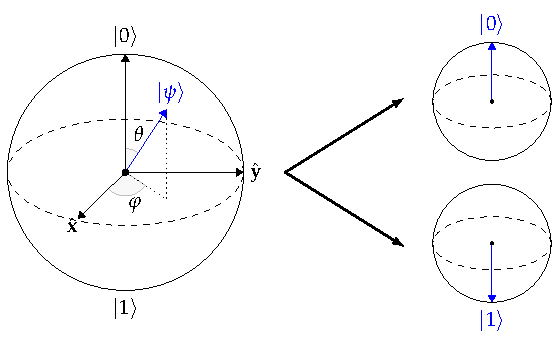
\includegraphics{Images/fig-qubitmeasurement.pdf}
    

    \caption{When we measure a qubit in the $S_z$ eigenbasis (in quantum information lingo, called the computational basis) of $\set{\ket{0}, \ket{1}}$, we only find one of two outcomes, and the post measurement-state is one of $\ket{0}, \ket{1}$ - one of two states, just like the classical bit (this is true regardless of what single-qubit measurement basis we choose; the possible post-measurement states will be some two antipodal points on the Bloch sphere).}
    \label{fig-qubitmeasurement}
\end{figure}

The answer to this question is illuminated by the discussion of our first (real!) quantum protocol - known as superdense coding. We will see in this protocol that it is possible to encode \emph{two} classical bits in a single qubit; provided we make use of entanglement. 

To discuss this protocol, we introduce the Bell basis - we have discussed the Bell state $\ket{B_{11}}$ already, but in fact there are four Bell states, which form a orthonormal basis (check!) for the Hilbert space of two qubits $\H = \CC^2 \otimes \CC^2$:
\begin{equation}
    \begin{split}
        \ket{B_{00}} &= \frac{\ket{0}\otimes \ket{0} + \ket{1} \otimes \ket{1}}{\sqrt{2}}
        \\ \ket{B_{01}} &= \frac{\ket{0}\otimes \ket{0} - \ket{1} \otimes \ket{1}}{\sqrt{2}}
        \\ \ket{B_{10}} &= \frac{\ket{0}\otimes \ket{1} + \ket{1} \otimes \ket{0}}{\sqrt{2}}
        \\ \ket{B_{11}} &= \frac{\ket{0}\otimes \ket{1} - \ket{1} \otimes \ket{0}}{\sqrt{2}}
    \end{split}
\end{equation}
Recalling that $\sigma_z = \dyad{0}{0} - \dyad{1}{1}$ and $\sigma_x = \dyad{0}{1} + \dyad{1}{0}$, we make the observation that the $01/10/11$ Bell states are related to the $00$ Bell state via the application of Paulis on the first qubit:
\begin{equation}\label{eq-BellstatePaulis}
    \begin{split}
        \ket{B_{01}} &= \sigma_{z, 1}\ket{B_{00}}
        \\ \ket{B_{10}} &= \sigma_{x, 1}\ket{B_{00}}
        \\ \ket{B_{11}} &= \sigma_{z, 1}\sigma_{x, 1}\ket{B_{00}}
    \end{split}
\end{equation}
Which we may summarize with the relation:
\begin{equation}
    \ket{B_{ab}} = (\sigma_{z, 1})^b(\sigma_{x, 1})^a\ket{B_{00}}.
\end{equation}
Note that we could very well have applied the Paulis to the second qubit, i.e.:
\begin{equation}
    \ket{B_{ab}} = (\sigma_{z, 2})^b(\sigma_{x, 2})^a\ket{B_{00}}.
\end{equation}
Although we will not need it for the superdense coding protocol (we will need it for the following teleportation protocol), it will be useful to note one more property of $\ket{B_{00}}$, namely that it is the $+1$ eigenvalue of $\sigma_z \otimes \sigma_z$ and $\sigma_x \otimes \sigma_x$ (check!):
\begin{equation}\label{eq-Bellstabilizers}
    \begin{split}
    \sigma_z \otimes \sigma_z \ket{B_{00}} &= \ket{B_{00}}
    \\ \sigma_x \otimes \sigma_x \ket{B_{00}} &= \ket{B_{00}}
    \end{split}
\end{equation}
Physically, this means that $S_z$ and $S_x$ measurements on the two qubits of $\ket{B_{00}}$ are perfectly correlated. It is also worth noting that $\ket{B_{00}}$ is uniquely specified by the property that it is so-called \emph{stabilized} by  $\sigma_z \otimes \sigma_z$ and $\sigma_x \otimes \sigma_x$ - this is probably the first time you have seen states described in this manner, but if you go on to do more courses/research in quantum information theory (and in particular quantum error correction) you will see this method of specifying states (via the operators they are stabilized by) come up time and time again through the \emph{stabilizer formalism}.


With this, we now have all the tools available to understand the superdense coding protocol, which we now lay out here.

\begin{blankbox}{Protocol: Superdense coding}
    \textbf{Objective:} Transmit two bits of information $a, b$ from $A$ to $B$. 

    \noindent
    \textbf{Protocol:}
    \begin{enumerate}
        \item In advance of the actual communication, the parties share a bell state $\ket{B_{00}}$ between themselves.
        \item Sender $A$ applies $(\sigma_z)^b(\sigma_x)^a$ to their qubit, encoding $(a, b) \in \ZZ_2 \times \ZZ_2$. 
        \item $A$ sends their qubit to $B$.
        \item $B$ measures their qubit in the Bell basis\footnote{Formally, they can measure some observable $O = \lambda_{00}\dyad{B_{00}}{B_{00}} + \lambda_{01}\dyad{B_{01}}{B_{01}} + \lambda_{10}\dyad{B_{10}}{B_{10}} + \lambda_{11}\dyad{B_{11}}{B_{11}}$, and since the state they have is one of the four Bell states, depending on which outcome $\lambda_{ab}$ they measure they can recover the two bits $a, b$.}. Depending on the outcome, they recover $a ,b$.
    \end{enumerate}
\end{blankbox}

So given the above protocol, is the answer that one qubit is worth two classical bits? The answer is not so clear cut - we would not have been able to transmit two bits of information had we only sent over an unentangled qubit. Indeed, the entanglement here played a role, and in communicating the two bits of information, we have used up one bit of entanglement.

Let us also discuss the counterpart to the superdense coding protocol - namely, the quantum teleportation protocol. In superdense coding, we wanted to communicate two bits worth of information and so we physically sent a qubit; in the teleportion protocol things are reversed; we will communicate/teleport a qubit state, and in order to do so physically send two classical bits worth of information. The protocol is as follows.

\begin{figure}[htbp]
    \centering
    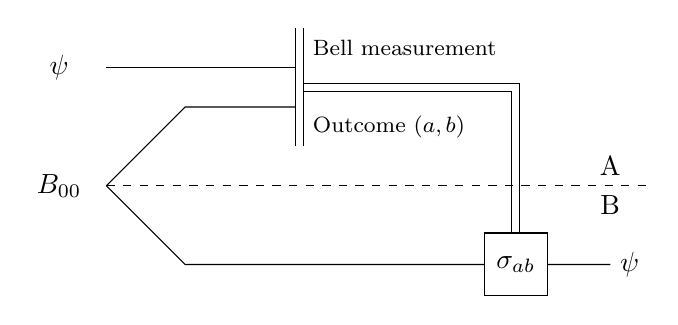
\begin{tikzpicture}
        \node[] at (0, 0) {$\ket{B_{00}}$};
        \draw[] (0.6, 0) -- (1.6, 1) -- (3, 1);
        \draw[] (0.6, 0) -- (1.6, -1) -- (7, -1);
        \draw[dashed] (0.6, 0) -- (7.5, 0);
        \draw[] (3, 2) -- (3, 0.5);
        \draw[] (3.1, 2) -- (3.1, 0.5);
        \node[above] at (7,0) {A};
        \node[below] at (7, 0) {B};
        \node[] at (0, 1.5) {$\ket{\psi}$};
        \draw[] (0.6, 1.5) -- (3, 1.5);
        \node[right] at (3.1, 1.75) {\footnotesize Bell measurement};
        \node[right] at (3.1, 0.75) {\footnotesize Outcome $(a, b)$};
        \node[right] at (7, -1) {$\ket{\psi}$};
        \filldraw[fill=white] (5.1+0.3, -0.6) -- (5.9+0.3, -0.6) -- (5.9+0.3, -1.4) -- (5.1+0.3, -1.4) -- cycle;
        \node[] at (5.8, -1) {$\sigma_{ab}$};
        \draw[] (3.1, 1.2) -- (5.75, 1.2) -- (5.75, -0.6);
        \draw[] (3.1, 1.3) -- (5.85, 1.3) -- (5.85, -0.6);
    \end{tikzpicture}
    \caption{Graphical depiction of the quantum teleportation protocol.}
    \label{fig-teleportation}
\end{figure}

\begin{blankbox}{Protocol: Quantum Teleportation}
    \textbf{Objective:} Transmit a qubit state $\ket{\psi} \in \CC^2$ from $A$ to $B$.

    \noindent
    \textbf{Protocol:}
    \begin{enumerate}
        \item In advance of the actual communication, the parties share a bell state $\ket{B_{00}}$ between themselves.
        \item $A$ prepares the state $\ket{\psi}$ she wants to transmit (she now has two qubits; one from the shared Bell pair, and one for $\ket{\psi}$).
        \item $A$ performs a measurement in the Bell basis on their two qubits, and obtains the two-bit outcome $(a, b)$. 
        \item $A$ transmits the two-bit measurement outcome $(a, b)$ to $B$.
        \item $B$ applies the correction operator $\sigma_{ab} = (\sigma_x)^a(\sigma_z)^b$ to their qubit. The resulting state of $B$'s qubit is $\ket{\psi}$.
    \end{enumerate}
\end{blankbox}

\noindent
\textit{Proof of Correctness.} Let $\ket{\psi} = \alpha\ket{0} + \beta\ket{1}$ be the state that $A$ wants to transmit to $B$. Let us label this qubit as qubit 1, $A$'s half of the Bell pair as qubit 2, and $B$'s half of the Bell pair as qubit 3. The initial state is then $\ket{\psi}_1 \otimes \ket{B_{00}}_{23}$. Now, we consider the action of the Bell measurement (with outcome $(a, b)$) on Alice's two qubits. Up to normalization, this has the effect of applying the projector:
\begin{equation}
    \Pi_{ab, 12} \otimes \II_3 = \dyad{B_{ab}}{B_{ab}}_{12} \otimes \II_3
\end{equation}
onto the state. Using Eq. \eqref{eq-BellstatePaulis}, we can write:
\begin{equation}
    \ket{B_{ab}}_{ij} = (\sigma_{z, i})^b(\sigma_{x, i})^a\ket{B_{00}}_{ij}
\end{equation}
and so we can rewrite the projector as:
\begin{equation}
    \Pi_{ab, 12} \otimes \II_3 = \dyad{B_{ab}}{B_{00}}_{12}(\sigma_{x, 2})^a(\sigma_{z, 2})^b \otimes \II_3
\end{equation}
So applying this to the initial state, we find:
\begin{equation}\label{eq-qteleportpart1}
    \begin{split}
        \Pi_{ab, 12} \otimes I_3\left(\ket{\psi}_1 \otimes \ket{B_{00}}_{23}\right) &= \left( \dyad{B_{ab}}{B_{00}}_{12}(\sigma_{x, 2})^a(\sigma_{z, 2})^b \otimes \II_3\right)\left((\alpha\ket{0}_1 + \beta\ket{1}_1) \otimes \ket{B_{00}}_{23}\right)
        \\ &=  \left( \dyad{B_{ab}}{B_{00}}_{12} \otimes \II_3\right) \left((\alpha\ket{0}_1 + \beta\ket{1}_1) \otimes ((\sigma_{x, 2})^a(\sigma_{z, 2})^b \otimes \II_3) \ket{B_{00}}_{23}\right)
    \end{split}
\end{equation}
Now using that $\ket{B_{00}}$ is stabilized by $\sigma_z \otimes \sigma_z$ and $\sigma_x \otimes \sigma_x$ (Equation \eqref{eq-Bellstabilizers}) we can write:
\begin{equation}
    \ket{B_{00}}_{23} = (\sigma_{z, 2} \otimes \sigma_{z, 3})^b\ket{B_{00}}_{23} = (\sigma_{z, 2} \otimes \sigma_{z, 3})^b(\sigma_{x, 2} \otimes \sigma_{x, 3})^a\ket{B_{00}}_{23}
\end{equation} 
And now using that $\sigma_i^2 = \II$ for each of the Pauli matrices:
\begin{equation}
    \begin{split}
        ((\sigma_{x, 2})^a(\sigma_{z, 2})^b \otimes \II_3)\ket{B_{00}}_{23} &= ((\sigma_{x, 2})^a(\sigma_{z, 2})^b \otimes \II_3)(\sigma_{z, 2} \otimes \sigma_{z, 3})^b(\sigma_{x, 2} \otimes \sigma_{x, 3})^a\ket{B_{00}}_{23}
        \\ &= ((\sigma_{x, 2})^a\otimes \II_3)((\sigma_{z, 2})^2 \otimes \sigma_{z, 3})^b(\sigma_{x, 2} \otimes \sigma_{x, 3})^a\ket{B_{00}}_{23}
        \\ &= ((\sigma_{x, 2})^a\otimes \II_3)(\II_2 \otimes \sigma_{z, 3})^b(\sigma_{x, 2} \otimes \sigma_{x, 3})^a\ket{B_{00}}_{23}
        \\ &= (\II_2 \otimes \sigma_{z, 3})^b((\sigma_{x, 2})^2\otimes \sigma_{x, 3})^a\ket{B_{00}}_{23}
        \\ &= (\II_2 \otimes \sigma_{z, 3})^b(\II_2 \otimes \sigma_{x, 3})^a\ket{B_{00}}_{23}
        \\ &= \II_2 \otimes (\sigma_{z, 3})^b(\sigma_{x, 3})^a \ket{B_{00}}_{23}
    \end{split}
\end{equation}
So then Eq. \eqref{eq-qteleportpart1} becomes:
\begin{equation}
    \begin{split}
        \Pi_{ab, 12} \otimes I_3\left(\ket{\psi}_1 \otimes \ket{B_{00}}_{23}\right) &= (\sigma_{z, 3})^b(\sigma_{x, 3})^a\left( \dyad{B_{ab}}{B_{00}}_{12} \otimes \II_3\right) \left(\ket{\psi}_1 \otimes \ket{B_{00}}_{23}\right)
        \\ &= (\sigma_{z, 3})^b(\sigma_{x, 3})^a\left( \frac{\dyad{B_{ab}}{00}_{12} + \dyad{B_{ab}}{11}_{12}}{\sqrt{2}} \otimes \II_3\right) \left(\frac{\alpha\ket{000}_{123} + \beta\ket{100}_{123} + \alpha\ket{011}_{123} + \beta\ket{111}_{123}}{\sqrt{2}}\right)
        \\ &= (\sigma_{z, 3})^b(\sigma_{x, 3})^a\frac{1}{2}\left(\ket{B_{ab}}_{12}\right) \otimes (\alpha\ket{0}_3 + \beta\ket{1}_3)
        \\ &= \frac{1}{2}\ket{B_{ab}}_{12} \otimes \left((\sigma_{z, 3})^b(\sigma_{x, 3})^a\ket{\psi}_3\right)
    \end{split}
\end{equation}
So indeed we have teleported $\ket{\psi}$ to the third ($B$'s) qubit, up to applying a correction operator of $\sigma_{ab} = (\sigma_{x, 3})^a(\sigma_{z, 3})^b$. 

\qed

Note that although the name might suggest some kind of superluminal communication, the teleportation protocol is fully consistent with special relativity - in order to recover the correct state $\ket{\psi}$ at the end, $A$ must transmit to $B$ the two-bit measurement outcome of the Bell basis measurement; this communication cannot exceed light speed.

A tangent to conclude this section that is certainly beyond the scope of this course but nevertheless interesting; a variant of the teleportation protocol (half-teleportation) forms the backbone of measurement-based quantum computation, where a computation is carried out solely via a sequence of local (adaptive) measurements on an initial resource state. You can read more about it \href{https://journals.aps.org/prl/pdf/10.1103/PhysRevLett.86.5188}{here}, among other places.

\subsection{Density Operators}
At the beginning of the course, we introduced the state ket in a Hilbert space $\ket{\psi} \in \H$ which represents a quantum state, and how it was a more abstract/general object than the wavefunction (which is nothing but the coefficients of the state ket expanded in a particular basis) $\psi(x)$ which was the primary objects of study in your first quantum mechanics course. However, it turns out that state kets are not the most general way of representing quantum states - the most general representation turns out to be density operators, and we give two examples (based on material already discussed in the course) as motivation for them.

The first example comes from the Stern-Gerlach experiment. Consider a stream of spin-1/2 particles where each spin is in the spin-up state with probability 1/2 and spin-down state with probability 1/2.How would we represent this physical situation?

Because it has a 50/50 probability of being measured to be up or down, we might consider the equal weight superposition of the $\ket{\uparrow}, \ket{\downarrow}$ states:
\begin{equation}\label{eq-unpolarizedguess}
    \ket{\psi} \stackrel{?}{=} \frac{\ket{\uparrow} + \ket{\downarrow}}{\sqrt{2}}
\end{equation}
We note that this is of course just the $S_x$ eigenstate of $\ket{\rightarrow}$. However, although this state indeed reproduces the correct measurement statistics for an $S_z$ measurement (where we get 50/50 outcomes), it must give the correct probabilities for any possible observable on the given physical system. To this end, we consider a measurement of $S_x$. By the laws of conditional probability, the probability of measuring spin right for a beam which has 50\% probability of being spin up or down should be:
\begin{equation}
    p(\rightarrow) = p(\uparrow)p(\rightarrow \vert \uparrow) + p(\downarrow)p(\rightarrow \vert \downarrow) = \frac{1}{2}\abs{\braket{\rightarrow}{\uparrow}}^2 + \frac{1}{2}\abs{\braket{\leftarrow}{\downarrow}}^2 = \frac{1}{2}\cdot \frac{1}{2} + \frac{1}{2} \cdot \frac{1}{2} = \frac{1}{2}
\end{equation}
In the above, $p(\uparrow/\downarrow)$ denotes the probability that the spin we draw from the beam is spin up or spin down, and $p(\rightarrow \vert \uparrow/\downarrow)$ denotes the probability that we measure spin-right given an input state of spin-up/spin-down. So, for our physical scenario, we have a probability of measuring spin-right of $\frac{1}{2}$. However for our guess of $\ket{\psi} = \ket{\rightarrow}$, of course $p(\rightarrow) = 1$ and so our guess is incorrect. We might try to refine our guess, but any such attempt will be futile. For the provided physical situation of the 50/50 up-down beam, we will have a 50/50 distribution of outcome no matter how we orient the Stern-Gerlach measurement appratus (check!) - however any state ket $\ket{\psi}$ will have to be an eigenstate of spin in some direction, and therefore will not be able to reproduce the measurement statistics for all possible observables. So, there is something that the state ket $\ket{\psi}$ cannot quite capture about this scenario.

The second example comes from our thought experiment of the entangled Bell pair, where one half of the Bell pair is taken to the moon while the other remains on Earth. Suppose I was the experimenter on Earth, and I want some description of the qubit on Earth only, from which I can derive all statistics of the measurements that I can do on it. In the state ket formalism, the fact that the state is entangled means that (by definition) I cannot associate any state ket to the Earth qubit alone. So we require a more general formalism to handle this scenario, as well\footnote{Although taking a qubit to the moon probably isn't of interest to most experimentalists, a more experimentally relevant and related scenario is when considering some system of interest and a larger, uncontrollable environment it is entangled with. In this case, we would want some way of just describing the system and deriving all measurement statistics of the system, somehow ignoring the larger environment it is coupled to.}.

Before jumping to what this generalization is, we first require one piece of mathematical machinery - namely, the \emph{trace} operation.

\begin{defbox}{: Trace}
    Let $A$ be any operator acting on a Hilbert space $\H$. The trace of $A$ is then defined as:
    \begin{equation}
        \Tr(A) \coloneqq \sum_i \bra{i}A\ket{i}
    \end{equation} 
    where the sum is taken over any ONB $\mathcal{B} = \set{\ket{i}}_{i=1}^{\dim(\H)}$. 
\end{defbox}

\begin{propbox}{: Properties of the trace}
    \begin{enumerate}
        \item The trace of $A$ is independent of the ONB chosen to evaluate it.
        \item The trace of $A$ is equal to the sum of eigenvalues of $A$. 
        \item The trace is cyclic, i.e. for operators $A, B, C$:
        \begin{equation}
            \Tr(ABC) = \Tr(BCA) = \Tr(CAB).
        \end{equation}
    \end{enumerate}
\end{propbox}
\begin{proof}
    \begin{enumerate}
        \item Let $\set{\ket{i}}_i, \set{\ket{j}}_j$ be two ONBs. We can express the $\ket{j}$s in terms of the $\ket{i}$s by:
        \begin{equation}
            \ket{j} = \sum_i \braket{i}{j} \ket{i}
        \end{equation}
        Taking the trace using the $\set{\ket{j}}_j$ ONB, we have:
        \begin{equation}
            \begin{split}
                \sum_j \bra{j}A\ket{j} &= \sum_j \left(\sum_i \braket{j}{i}\bra{i}\right)A\left(\sum_{i'}\braket{i'}{j}\ket{i'}\right)
                \\ &= \sum_{i, i'} \left(\bra{i'} \left(\sum_j \dyad{j}{j} \right)\ket{i}\right) \bra{i}A\ket{i'}
                \\ &= \sum_{i, i'} \left(\bra{i'} \II \ket{i}\right) \bra{i}A\ket{i'}
                \\ &= \sum_{i, i'} \braket{i'}{i}\bra{i}A\ket{i'}
                \\ &= \sum_{i, i'}\delta_{ii'}\bra{i}A\ket{i'}
                \\ &= \sum_i \bra{i}A\ket{i}
            \end{split}
        \end{equation}
        where in the third equality we use the resolution of the identity. Hence the trace evaluated using the two ONBs are equivalent, proving the claim.
        \item Take $\mathcal{B}$ to be the eigenbasis of $A$; the claim immediately follows. 
        \item First, we show that $\Tr(AB) = \Tr(BA)$ for two operators $A, B$. Let $C = AB$ and $D = BA$. Consider some ONB $\set{\ket{i}}_i$. Inserting the resolution of the identity, we have:
        \begin{equation}
            \begin{split}
                \bra{i}C\ket{j} &= \sum_m \bra{i}A \dyad{m}{m}B\ket{j}
                \\ \bra{i}D\ket{j} &= \sum_m \bra{i}B\dyad{m}{m}A\ket{j}
            \end{split}
        \end{equation}
        And so taking the trace of $C$:
        \begin{equation}
            \begin{split}
                \Tr(C) &= \sum_i \bra{i}C\ket{i}
                \\ &= \sum_i \sum_m \bra{i}A \dyad{m}{m}B\ket{i}
                \\ &= \sum_i \sum_m \bra{m}B\ket{i}\bra{i}A\ket{m}
                \\ &= \sum_m \sum_i \bra{m}B\ket{i}\bra{i}A\ket{m}
                \\ &= \sum_m \bra{m}D\ket{m}
                \\ &= \Tr(D)
            \end{split}
        \end{equation}
        So $\Tr(C) = \Tr(D)$. To prove $\Tr(ABC) = \Tr(BCA)$, take $A \to A, B \to BC$ in the above, and to prove $\Tr(BCA) = \Tr(CAB)$, take $A \to B, B \to CA$ in the above. 
    \end{enumerate}
\end{proof}

Now that we've discussed the trace, we can move on to constructing and defining the density operator. Consider an ensemble $\mathcal{E}$ of states $\ket{\phi_i}$ drawn rnadomly, with probabilities $p_i$ (e.g. in the Stern-Gerlach motivating example, drawing $\ket{\uparrow}$ with $p_\uparrow = \frac{1}{2}$ and $\ket{\downarrow}$ with $p_\downarrow = \frac{1}{2}$)"
\begin{equation}
    \mathcal{E} = \set{(p_i, \ket{\phi_i})}_i
\end{equation}
Given $\mathcal{E}$, for any operator $A$, the expectation $\avg{A}_\mathcal{E}$ is:
\begin{equation}
    \avg{A}_\mathcal{E} = \sum_i p_i \bra{\phi_i}A\ket{\phi_i}
\end{equation}
i.e. the sum of expectation values for the states in the ensemble, weighted by the probability of drawing them. Let us manipulate this expression by inserting the resolution of the identity:
\begin{equation}
    \begin{split}
        \avg{A}_\mathcal{E} &= \sum_i p_i \bra{\phi_i}A\ket{\phi_i}
        \\ &= \sum_i p_i \sum_j \braket{\phi_i}{j}\bra{j}A\ket{\phi_i}
        \\ &= \sum_i p_i \sum_j \bra{j}A\ket{\phi_i}\braket{\phi_i}{j}
        \\ &= \sum_i p_i \Tr(A\dyad{\phi_i}{\phi_i})
        \\ &= \Tr(A\left[\sum_i p_i \dyad{\phi_i}{\phi_i}\right])
        \\ &= \Tr(A\rho)
    \end{split}
\end{equation}
where in the last equality we define the density operator $\rho = \sum_i p_i \dyad{\phi_i}{\phi_i}$. The density operator corresponding to an ensemble contains all the physically relevant information that the ensemble contains (e.g. all relevant statistics of measurement and evolution can be done with the density operator). It is worth noting however that a given density operator does not correspond to a unique ensemble (can you show this by example?)

\begin{defbox}{: Density Operators}
    For any ensemble $\mathcal{E} = \set{(p_i, \ket{\phi_i})}_i$,
    \begin{equation}
        \rho \coloneqq \sum_i p_i \dyad{\phi_i}{\phi_i}
    \end{equation}
    is the corresponding density operator.
\end{defbox}

\begin{propbox}{: Density Operator Properties}
    For all density operators $\rho$ it holds that:
    \begin{enumerate}
        \item $\Tr(\rho) = 1$ (Normalization)
        \item $\rho^\dag = \rho$ (Hermicity)
        \item $\bra{\psi}\rho\ket{\psi} \geq 0, \quad \forall \ket{\psi} \in \H$ (Positivity)
    \end{enumerate}
\end{propbox}
\begin{proof}
    Left as a homework exercise.
\end{proof}

\begin{defbox}{: Pure and Mixed States}
    If a density operator $\rho$ has a single eigenvalue of $1$ and all other eigenvalues $0$, it is called pure, and $\rho = \dyad{\phi}{\phi}$. Otherwise, it is called mixed.
\end{defbox}

Note that pure operators $\rho = \dyad{\phi}{\phi}$ correspond to state kets $\ket{\phi}$. However, the density operator formalism is able to account for probabilistic mixtures (mixed states) which was not something that state kets were able to represent.

\begin{propbox}{: Criterion for purity}
    All density operators $\rho$ satisfy $\Tr(\rho^2) \leq 1$, with equality if and only if $\rho$ is pure.
\end{propbox}

\begin{proof}
    Left as homework exercise.
\end{proof}

\begin{axiombox}{: Quantum measurement (with density operators)}
    Consider a measurement with corresponding projectors $\mathcal{M} = \set{\Pi_i, i = 1, \ldots k}$ on a density operator $\rho$. 

    \noindent
    \textbf{Dirac postulate:} When we measure outcome $i$, the density operator evolves as:
    \begin{equation}
        \rho \mapsto \frac{\Pi_i \rho \Pi_i}{\Tr(\Pi_i \rho)}
    \end{equation}

    \noindent \textbf{Born rule:} The probability of measuring outcome $i$ is given by:
    \begin{equation}
        p(i) = \Tr(\Pi_i \rho).
    \end{equation}
\end{axiombox}

\begin{axiombox}{: Unitary evolution (with density operators)}
    Considering the time-dependent Schr\"{o}dinger equation as a PDE for time-evolution operators:
    \begin{equation}
        i\hbar\dpd{}{t}U(t, t_0) = HU(t, t_0)
    \end{equation}
    with $U(t_0, t_0) = \II$. Density operators evolve as:
    \begin{equation}
        \rho(t) = U(t, t_0)\rho(t_0)U^\dag(t, t_0)
    \end{equation}
    or expressed in terms of a PDE:
    \begin{equation}
        i\hbar\dpd{}{t}\rho(t) = [H, \rho(t)].
    \end{equation}
\end{axiombox}

You can verify that when $\rho$ is a pure state, the Dirac postulate/Born rule/Unitary evolution stated in the density operator formalism reduces to the familiar axioms for measurement/unitary evolution of state kets.

To close out this section, we return to the motivating example; how do we represent the state corresponding to a beam of spin-1/2 particles where each spin in the beam is spin-up with probability 1/2 and spin-down with probability 1/2? Note that this scenario is precisely what you encountered in the first homework assignment; there, we fed a beam of spin-right particles into a Stern-Gerlach apparatus that measured the $z$-component of spin (so by the Born rule there is a 50/50 distribution of outcome for measuring spin-up/spin-down) and then we recombined the two up/down beams such that we ``forgot'' the measurement outcome for a given individual spin in the final combined beam.

The answer is that we have a mixed state; the ensemble corresponding to the beam in this scenario is $\set{(\frac{1}{2}, \ket{\uparrow}), (\frac{1}{2}, \ket{\downarrow})}$. If we then calculate the corresponding density operator, we find:
\begin{equation}
    \rho_{50/50} = \frac{1}{2}\dyad{\uparrow}{\uparrow} + \frac{1}{2}\dyad{\downarrow}{\downarrow} \cong \frac{1}{2}\m{1 & 0 \\ 0 & 1}.
\end{equation}
Compare this to the density operator corresponding to the incoming beam, which is a pure state:
\begin{equation}
    \rho_\rightarrow = \dyad{\rightarrow}{\rightarrow} \cong \frac{1}{2}\m{1 & 1 \\ 1 & 1}
\end{equation}
Note that in both cases we have represented the density operator in the $S_z$ eigenbasis, under the identification $\ket{\uparrow} \cong \binom{1}{0}$ and $\ket{\downarrow} \cong \binom{0}{1}$. We make a key observation - in the case of $\rho_\rightarrow$, we have non-vanishing off-diagonal entries. The meaning of these off-diagonal elements is the coherences in between the two basis states we are expanding in. In the case of $\rho_\rightarrow$, we have a coherent superposition between $\ket{\uparrow}, \ket{\downarrow}$ (namely - $\ket{+} = \frac{\ket{\uparrow} + \ket{\downarrow}}{\sqrt{2}}$) and so the off-diagonals have maximal magnitude. In the  case of $\rho_{50/50}$, the off-diagonals are zero\footnote{Some terminology - in the cases where $\rho \propto \mathbb{I}$, we say that we have a maximally mixed state. In this case there is no coherence between the basis states whatsoever.}, indicating that we have a decoherent mixture of the two basis states $\ket{\uparrow}, \ket{\downarrow}$.

In conclusion, let us quickly summarize what the meaning of the density matrix elements are (when represented in some ONB $\mathcal{B} = \set{\ket{i}}_i$). The diagonal entries $[\rho]_{ii} = \bra{i}\rho\ket{i}$ tells us about the probability of obtaining the basis state $\ket{i}$ if we conduct a measurement of $\rho$ in the basis $\mathcal{B}$. The diagonal entries $[\rho]_{ij} = \bra{i}\rho\ket{j}$ give us information about the coherences between the states $\ket{i}, \ket{j}$ in the basis.

\subsection{Reduced Density Operators and Impossibility of Superluminal Communication}
We've seen how density operators can handle probabilistic (decoherent) mixtures; in this section we will see how they are able to handle describing some portion of a larger (potentially entangled) state, as in the Bell state between Earth and Moon scenario.

We will require one more piece of mathematical machinery before jumping into it though; namely, the \emph{partial trace}.

\begin{defbox}{: Partial trace}
    Consider an operator $X_{AB}$ acting on a composite Hilbert space $\H_A \otimes \H_B$. Let $\mathcal{B}_A = \set{\ket{i}, i = 1, \ldots, d_A}, \mathcal{B}_B = \set{\ket{j}, j = 1, \ldots, d_B}$ be ONBs on $A/B$. Then, the partial trace $\Tr_A(X_{AB})$ is defined as:
    \begin{equation}
        \Tr_A(X_{AB}) \coloneqq \sum_i^{d_A} \prescript{}{A}{\bra{i}}X_{AB}\ket{i}_A
    \end{equation}
    where the sum is taken over $\mathcal{B}_A$. $\Tr_B(X_{AB})$ is defined analogously.
\end{defbox}

This definition requires some parsing - it is not immediately clear how an operator $X_{AB}$ which acts on the composite Hilbert space $\H_A \otimes \H_B$ acts on a basis ket $\ket{i}$ of $\H_A$. To this end, we note that the pairwise tensor products of states from $\mathcal{B}_A$ and $\mathcal{B}_B$ form a basis for $\H_A \otimes \H_B$. So, we can insert two resolutions of the identity:
\begin{equation}
    X_{AB} = \sum_{k, r}^{d_A} \sum_{l, s}^{d_B} \ket{k}_A\bra{k} \otimes \ket{l}_B\bra{l} X_{AB}\ket{r}_A\bra{r} \otimes \ket{s}_B\bra{s}
\end{equation}
We also observe that:
\begin{equation}
    \prescript{}{A}{\bra{i}}\left(\ket{k}_A \otimes \ket{l}_B\right) = \braket{i}{k}_A \ket{l}_B = \delta_{ik}\ket{l}_B
\end{equation}
Therefore, with respect to these bases:
\begin{equation}
    \begin{split}
        \Tr_A(X_{AB}) &= \sum_i^{d_A} \prescript{}{A}{\bra{i}} \left(\sum_{k, r}^{d_A} \sum_{l, s}^{d_B} \ket{k}_A\bra{k} \otimes \ket{l}_B\bra{l} X_{AB}\ket{r}_A\bra{r} \otimes \ket{s}_B\bra{s}\right)\ket{i}_A
        \\ &= \sum_{i, k, r}^{d_A}\sum_{l, s}^{d_B} \delta_{ik}\ket{l}_B\left(\prescript{}{A}{\bra{k}} \otimes \prescript{}{B}{\bra{l}}X_{AB}\ket{r}_A \otimes \ket{s}_B\right)\prescript{}{B}{\bra{s}}\delta_{ir}
        \\ &= \sum_{i}^{d_A}\sum_{l, s}^{d_B} \ket{l}_B\left(\prescript{}{A}{\bra{i}} \otimes \prescript{}{B}{\bra{l}}X_{AB}\ket{i}_A \otimes \ket{s}_B\right)\prescript{}{B}{\bra{s}}
    \end{split}
\end{equation}
Note that partial traces have the following important property (which we state without proof, but if you are able to parse the definition of the partial trace, it should follow from the definition without too much trouble):
\begin{propbox}{: Trace and partial trace}
    Let $X_{AB}$ be an operator on the composite Hilbert space $\H_A \otimes \H_B$. Then:
    \begin{equation}
        \Tr(X) = \Tr_B(\Tr_A(X_{AB})) = \Tr_A(\Tr_B(X_{AB})).
    \end{equation}
\end{propbox}

We also note that the partial trace, like the trace has a cyclicity property (although weaker):
\begin{propbox}{: Cyclicity of partial trace}
    Let $X_{AB}$ be an operator acting on a composite Hilbert space $\H_A \otimes \H_B$ and let $T_A, S_A$ be operators acting on $\H_A$. Then:
    \begin{equation}
        \Tr_A([T_A \otimes I_B] X_{AB} [S_A \otimes I_B]) = \Tr_A([S_AT_A \otimes I_B]X_{AB}).
    \end{equation}
\end{propbox}



We now construct the \emph{reduced density operator}. Consider any observable $O_A \otimes I_B$ (i.e. where we have some observable of interest on $A$ only - you can think of $A$ as the Earth and $B$ as the moon in the Earth-Moon Bell state scenario). Consider an arbitrary bipartite state $\ket{\psi}_{AB}$. Calculating the expectation value of $O_A \otimes I_B$ with respect to this state, we have:
\begin{equation}
    \begin{split}
        \avg{O_A \otimes I_B}_\psi &= \Tr(O_A \otimes I_B \ket{\psi}_{AB}\bra{\psi})
        \\ &= \Tr_A(\Tr_B(O_A \otimes I_B \ket{\psi}_{AB}\bra{\psi}))
        \\ &= \Tr_A(O_A \Tr_B(\ket{\psi}_{AB}\bra{\psi}))
        \\ &= \Tr_A(O_A\rho_A)
    \end{split}
\end{equation}
where in the first equality we take the expectation value in the density operator formalism (with $\rho_{AB} = \ket{\psi}_{AB}\bra{\psi}$), in the second equality we use that $\Tr(\cdot) = \Tr_A(\Tr_B(\cdot))$ as in the above proposition, and in the final equality we define $\rho_A \coloneqq \Tr_B(\ket{\psi}_{AB}\bra{\psi})$ as the reduced density operator on subsystem $A$.

\begin{defbox}{: Reduced density operator}
    Given a quantum state (density operator) $\rho_{AB}$ acting on a composite Hilbert space $\H_A \otimes \H_B$, the reduced density operator on subsystem $A$ is given by:
    \begin{equation}
        \rho_A \coloneqq \Tr_B(\rho_{AB})
    \end{equation}
\end{defbox}

By tracing out the $B$ subsystem, we are able to obtain an object (the reduced density operator - which itself is a density operator) that contains all information about the statistics we would obtain from operations we perform on subsystem $A$ only. Note that (crucially) this formalism still applies even if the joint quantum state $\rho_{AB}$ is entangled (that is, $\rho_{AB} \neq \rho_1 \otimes \rho_2$ for any $\rho_1, \rho_2$). 

Using the formalism of reduced density operators, we are able to prove the following:

\begin{thmbox}{: No superluminal communication}
    Quantum mechanics does not provide for superluminal communication.
\end{thmbox}

We previously ruled out one proposed protocol on the basis of the no-cloning theorem; here we prove that any such proposed protocol is destined to fail.

\begin{proof}
    Consider any state $\rho_{AB}$ shared between parties $A$ and $B$. We prove that superluminal communication is impossible by showing that it is impossible for a local operation at $A$ to change the reduced density operator on subsystem $B$:
    \begin{equation}
        \rho_B \coloneqq \Tr_A(\rho_{AB}).
    \end{equation}
    In order to do this, we show that no form of quantum mechanical evolution on subsystem $A$ can change $\rho_B$; in other words, we show that it is (i) impossible for local unitary evolution on subsystem $A$ to change $\rho_B$ and (ii) local measurement on subsystem $A$ to change $\rho_B$. 

    \begin{enumerate}[(i)]
        \item (Unitary Evolution). Unitary evolution on $A$ evolves $\rho_{AB}$ as:
        \begin{equation}
            \rho_{AB} \mapsto (U_A \otimes I_B)\rho_{AB}(U^\dag_A \otimes I_B)
        \end{equation}
        But we observe:
        \begin{equation}
            \Tr_A((U_A \otimes I_B)\rho_{AB}(U^\dag_A \otimes I_B)) = \Tr_A((U^\dag_A \otimes I_B)(U_A \otimes I_B)\rho_{AB}) = \Tr_A(\rho_{AB}) = \rho_B
        \end{equation}
        where we use the cyclicity of the partial trace. We conclude that $\rho_B$ is unchanged by local unitary evolution on subsystem $A$. 
        \item (Measurement). We consider a measurement on $A$ from the perspective of $B$. Since $B$ doesn't know the outcome of the measurement, $\rho_{AB}$ is replaced with the average over all possible measurement outcomes:
        \begin{equation}
            \rho_{AB} \mapsto \sum_i \frac{(\Pi_{i, A} \otimes I_B)\rho_{AB}(\Pi_{i, A} \otimes I_B)}{\Tr(\Pi_{i, A}\rho_{AB})}\Tr(\Pi_{i, A}\rho_{AB}) = \sum_i(\Pi_{i, A} \otimes I_B)\rho_{AB}(\Pi_{i, A} \otimes I_B)
        \end{equation}
        where the $\frac{(\Pi_{i, A} \otimes I_B)\rho_{AB}(\Pi_{i, A} \otimes I_B)}{\Tr(\Pi_{i, A}\rho_{AB})}$ comes from the Dirac postulate in the density operator formalism, and the $\Tr(\Pi_{i, A}\rho_{AB})$ is the weight in the average. Now tracing out subsystem $A$, we have:
        \begin{equation}
            \Tr_A(\sum_i(\Pi_{i, A} \otimes I_B)\rho_{AB}(\Pi_{i, A} \otimes I_B)) = \Tr_A(\sum_i \Pi_{i, A}^2 \otimes I_B \rho_{AB}) = \Tr_A(\rho_{AB}) = \rho_B
        \end{equation} 
        where we have again used the cyclicity of the partial trace, as well as the completeness relation for projectors. We conclude that local measurement on subsystem $A$ does not change $\rho_B$. 
    \end{enumerate}
\end{proof}


\subsection{Quantum Cryptography}
There are many instances (e.g. protecting your credit card information for an online transaction) in which we require secure communication - where the information is only accessible to the sender and recipient, and inaccessible to potential eavesdroppers. On the end of cryptographic protocols, we have two desiredata:
\begin{enumerate}[(a)]
    \item The protocols are \emph{unconditionally secure} - that is, the security of the protocol is based on the laws of physics/information theory.
    \item The protocols are \emph{practical} - that is, they can be carried out via local operations and (potentially quantum) communication.
\end{enumerate} 

\begin{table}[htbp]
    \centering\begin{tabular}{|c|c|c|}
        \hline & Impractical & Practical
        \\ \hline Secure & Classical & Quantum
        \\ \hline Insecure & (Undesirable) & Classical
        \\ \hline
    \end{tabular}
    \caption{Feasibility of cryptography using classical/quantum resources. With classical cryptography, we have secure but impractical protocols, and practical but insecure protocols. Quantum resources are able to provide protocols which are both secure and practical.}
    \label{fig-cryptography}
\end{table}

Before moving into quantum protocols, we look at some classical counterparts.

\begin{blankbox}{Protocol: One-time pad}
    \textbf{Objective:} To (securely) send a bitstring $\v{x}$ from $A$ to $B$.

    \noindent
    \textbf{Protocol:}
    \begin{enumerate}
        \item The communicating parties $A$ and $B$ share a random bit string $\v{r}$ (for simplicitly - the message $\v{x}$ and the bitstring $\v{r}$ contain the same number of bits), e.g.:
        \begin{equation}
            \v{r} = (00010101001010010100011100\ldots)
        \end{equation}
        That is, $A$ holds a copy of $\v{r}$ and $B$ does too.
        \item $A$ computes:
        \begin{equation}
            \v{c} \coloneqq \v{x} \oplus \v{r}
        \end{equation}
        where $\oplus$ denotes component-wise addition modulo 2 (i.e. $0 + 0 = 1 + 1 = 0, 0 + 1 = 1 + 0 = 1$ for each component of the bitstring), and broadcasts $\v{c}$ to the world.
        \item $B$ receives the encoded message $\v{c}$, and computes:
        \begin{equation}
            \v{c} \oplus \v{realm} = \v{x} \oplus \v{r} \oplus \v{r} = \v{x}.
        \end{equation}
        The message $\v{x}$ is thus successfully transmitted.
    \end{enumerate}
\end{blankbox}
The one-time pad is secure, but impractical - the impracticality arises from the necessity of having a shared random bitstring $\v{r}$. Of course one cannot repeatedly use the same bitstring to encode information, as then the code could be broken (hence - the ``one-time'' pad). Therefore, at some point one runs of randomly shared bitstring, and information cannot be communicated securely any longer.

We now consider a classical protocol in the other quadrant of Table \ref{fig-cryptography}.

\begin{blankbox}{Protocol: RSA (Sketch)}
    \textbf{Objective:} To (securely) send a bitstring $\v{x}$ from $A$ to $B$.

    \noindent
    \textbf{Protocol:}
    \begin{enumerate}
        \item $B$ chooses two prime numbers $m, n$ and broadcasts $m \cdot n$.
        \item $A$ uses $m \cdot n$ as a key to encode the message $\v{x}$, and broadcasts $m \cdot n(\v{x})$. 
        \item $B$ receives and decodes the encoded message $m\cdot n(\v{x})$ using $m, n$.
    \end{enumerate}

    The full protocol in detail can be found \href{https://en.wikipedia.org/wiki/RSA_(cryptosystem)}{here}.
\end{blankbox}
Why is this protocol not unconditionally secure? It is because it rests on the computational assumption that factoring $m \cdot n$ into the prime factors $m, n$ is computationally hard - it is widely believed that there exists no polynomial time algorithm for prime factorization\footnote{at least classically - Shor's celebrated quantum algorithm is a polynomial time algorithm for prime factorization, but it requires a quantum computer. So, quantum computers are able to break RSA. Stay tuned for the end of the chapter for some discussion.}; however this has not been proven. There is no physical or information theoretic law guaranteeing its security.

We now discuss a quantum cryptographic protocol which is both unconditionally secure and practical.

\begin{blankbox}{Protocol: BB84}
    \textbf{Objective:} To (securely) send a bitstring $\v{x}$ from $A$ to $B$.

    \noindent
    \textbf{Protocol:}
    \begin{enumerate}
        \item $B$ the communicating parties $A, B$ share a large number of Bell states $\ket{B_{00}}^{\otimes n}$.
        \item $A$ and $B$ randomly measure their halves of Bell pairs either in the $Z$ or $X$ basis.
        \item $A$ and $B$ make public their choices of measurement bases (not outcomes).
        \item The measurement outcomes on the qubit pairs where the measurement bases agreed form the key. Of this key, $B$ publishes a small subset of bits.
        \item $A$ compares the measurement outcomes published by $B$ to her own. If there is perfect agreement, the remainder of the key is kept. Otherwise, the protocol is aborted (Note: not establishing communication is not a failure, only being eavesdropped is).
        \item The key obtained by the above can now be used to send $\v{x}$ from $A$ to $B$ securely, using the one-time pad protocol.
    \end{enumerate}
\end{blankbox}

Let's study each step of this protocol. In the first step, we have the sharing of a large number of Bell states $\ket{B_{00}}_{AB} = \frac{\ket{0}_A \otimes \ket{0}_B +  \ket{1}_A \otimes \ket{1}_B}{\sqrt{2}}$. Why these states in particular? We recall the property (Eq. \eqref{eq-Bellstabilizers}) that $Z$ and $X$ measurements are perfectly correlated\footnote{Since $\ket{B_{11}}$ displays strict anti-correlation of measurement outcomes in any local measurement basis, one might ask then whether $\ket{B_{00}}$ displays strict correlation of measurement outcomes in every local measurement basis. The answer turns out to be no - moreover, no bipartite state can display perfect correlation in every local measurement basis. Can you show it?} for $\ket{B_{00}}$. So, if we do an $X$ measurement, we have the post measurement states:
\begin{equation}
    \begin{split}
        \text{outcome ``+'': } \ket{B_{00}}_{AB} &\to \ket{+}_A \otimes \ket{+}_B
        \\ \text{outcome  ``-'': } \ket{B_{00}}_{AB} &\to \ket{-}_A \otimes \ket{-}_B
    \end{split}
\end{equation}
where $\ket{\pm} = \frac{\ket{0} \pm \ket{1}}{\sqrt{2}}$ are the usual $S_x$ eigenstates (with some new notation, commonly used in the quantum information literature). If we do an $Z$ measurement, we instead get the outcomes:
\begin{equation}
    \begin{split}
        \text{outcome ``+'': } \ket{B_{00}}_{AB} &\to \ket{0}_A \otimes \ket{0}_B
        \\ \text{outcome  ``-'': } \ket{B_{00}}_{AB} &\to \ket{1}_A \otimes \ket{1}_B
    \end{split}
\end{equation}
So, in the second step where Alice/Bob measure their halves of Bell pairs in the $Z$ or $X$ basis, if the measurement bases agree then they will see strict correlation of measurement outcomes, and if the measurement bases disagree then they will see no correlation.

We give an example of steps 3-5 in Table \ref{table-BB84} below.

\begin{table}[htbp]
    \centering\begin{tabular}{|c|c|c|c|c|c|c|c|c|c|c|}
         \hline Bases & 1 & 2 & 3 & 4 & 5 & 6 & 7 & 8 & 9
         \\ \hline A & \textcolor{red}{X} & \textcolor{green}{Z} & \textcolor{green}{X} & \textcolor{green}{Z} & \textcolor{green}{Z} & \textcolor{red}{Z} & \textcolor{green}{X} & \textcolor{red}{Z} & \textcolor{red}{X} 
         \\ \hline B & \textcolor{red}{Z} & \textcolor{green}{Z} & \textcolor{green}{X} & \textcolor{green}{Z} & \textcolor{green}{Z} & \textcolor{red}{X} & \textcolor{green}{X} & \textcolor{red}{X} & \textcolor{red}{Z} 
         \\ \hline Outcomes & 1 & \textcolor{blue}{2} & \textcolor{pink}{3} & \textcolor{pink}{4} & \textcolor{pink}{5} & 6 & \textcolor{blue}{7} & 8 & 9 
         \\ \hline A & \textcolor{red}{+} & \textcolor{green}{-} & \textcolor{green}{+} & \textcolor{green}{+} & \textcolor{green}{-} & \textcolor{red}{-} & \textcolor{green}{+} & \textcolor{red}{-} & \textcolor{red}{+} 
         \\ \hline B & \textcolor{red}{+} & \textcolor{green}{-} & \textcolor{green}{+} & \textcolor{green}{+} & \textcolor{green}{-} & \textcolor{red}{+} & \textcolor{green}{+} & \textcolor{red}{-} & \textcolor{red}{-} 
         \\ \hline
    \end{tabular}
    \caption{$A$ and $B$ publicly publish their measurement bases (step 3), and see which ones agree (green) - the bell pairs for which the measurement bases disagree (red) are discarded. $B$ then publishes a small subset of his measurement results (here, results -+ from 2/7, blue) for which the bases agreed (step 4). If $A$ and $B$ agree on the measurement outcomes for those, then the key consisting of the remaining measurement outcomes for which the bases agree (here ++- (001) from 3/4/5, pink) is kept and can be used for a one-time pad protocol.}
    \label{table-BB84}
\end{table}

The protocol works as if is no eavesdropping, the measurement outcomes for which the measurement bases are the same should agree (and this is checked via $B$ publishing a subset of his measurement outcomes for which the bases are the same), and then the remainder of the outcomes is unknown to the world (only the bases are known) while $A$/$B$ share it in confidence.

Let us explore one strategy that an eavesdropper $E$ might take to eavesdrop on the key, and show why the strategy fails. In step 1 of the protocol, suppose $E$ intercepts the Bell states shared between $A$ and $B$ and entangles herself with them:
\begin{equation}
    \ket{B_{00}}_{AB} = \frac{\ket{0}_A \otimes \ket{0}_B + \ket{1}_A \otimes \ket{1}_B}{\sqrt{2}} \mapsto \frac{\ket{0}_A \otimes \ket{0}_B \otimes \ket{0}_E + \ket{1}_A \otimes \ket{1}_B \otimes \ket{1}_E}{\sqrt{2}} \eqqcolon \ket{GHZ}_{ABE}
\end{equation}
where the rightmost state is what is known as the Greenberger-Horne-Zeilinger state. Now, if $A$ and $B$ measure in the $Z$ basis ($\set{\ket{0}, \ket{1}}$), we have:
\begin{equation}
    \begin{split}
        \text{outcome ``+'': } \ket{GHZ}_{ABE} &\to \ket{0}_A \otimes \ket{0}_B \otimes \ket{0}_E
        \\ \text{outcome  ``-'': } \ket{GHZ}_{ABE} &\to \ket{1}_A \otimes \ket{1}_B \otimes \ket{1}_E
    \end{split}
\end{equation}
So $E$ learns of the measurement outcome, and therefore the key! However, if $A$ and $B$ measure in the $X$ basis ($\set{\ket{+}, \ket{-}}$), what happens? Let's work it out. First, the full density operator corresponding to the GHZ state is:
\begin{equation}
    \rho_{ABE} = \ket{GHZ}_{ABE}\bra{GHZ} = \frac{\ket{000}_{ABE}\bra{000} + \ket{000}_{ABE}\bra{111} + \ket{111}_{ABE}\bra{000} + \ket{111}_{ABE}\bra{111}}{2}
\end{equation}
so tracing over Eve's qubit:
\begin{equation}
    \rho_{AB} = \Tr_E(\rho_{ABC}) = \prescript{}{E}{\bra{0}}\rho_{ABE}\ket{0}_E + \prescript{}{E}{\bra{1}}\rho_{ABE}\ket{1}_E = \frac{\ket{00}_{AB}\bra{00} + \ket{11}_{AB}\bra{11}}{2}
\end{equation}
And so if we calculate $\avg{\sigma_{x, A} \otimes \sigma_{x, B}}$, we find:
\begin{equation}
    \avg{\sigma_{x, A} \otimes \sigma_{x, B}} = \Tr((\sigma_{x, A} \otimes \sigma_{x, B})\rho_{AB}) = \Tr(\frac{\ket{00}_{AB}\bra{11} + \ket{11}_{AB}\bra{00}}{2}) = 0.
\end{equation}
So, we find that $X$-measurements of $A$ and $B$ are uncorrelated! However, $A$ and $B$ know that if they both measure the bell state $\ket{B_{00}}$ in the $X$-basis that the measurement outcomes should be perfectly correlated. Therefore, when they find that the measurements are uncorrelated (in step 5 of the protocol) Eve would be detected, and the protocol would be aborted.

Specifically: for each Bell state $\ket{B_{00}}$ that $E$ entangles herself with (that gets used in step 4; i.e. for each Bell state that $A/B$ measure in the same basis for, and for which $B$ publishes the measurement outcomes publicly), she learns a bit of information with probability $\frac{1}{2}$ (she learns 1 bit if $A$/$B$ measure in $Z$, and nothing if $A$/$B$ measure in $X$). So, for each Bell pair, $E$ can be said to learn half a bit of information. What is the probability of $E$ being detected? Well, if $A/B$ measure in the $Z$ basis (which occurs with probability $\frac{1}{2}$ since they pick randomly from $Z/X$), then $E$ is undetected. If $A/B$ measure in the $X$ basis (probability $1/2$) then the measurement outcomes are uncorrelated; so 50\% of the time they will measure the same outcome and not detect $E$ eavesdropping, and 50\% of the time they measure different outcomes and detect $E$ eavesdropping. So, for each Bell pair, the probability of $E$ being detected is $\frac{1}{2} \cdot \frac{1}{2} = \frac{1}{4}$.

In other words, for each half bit of information $E$, there is probability $\frac{1}{4}$ for $E$ to be detected. So, if $E$ learns $n$ bit of information, the probability they are not detected is $\left(\frac{3}{4}\right)^{2n} = \left(\frac{9}{16}\right)^{n}$ so the probability of $E$ not being detected decays exponentially in the number of bits that they learn. So, the protocol is secure against this kind of eavesdropping. This concludes our discussion of perhaps the most accessible near-term application of quantum entanglement. Time permitting, we will discuss another application - quantum computation - at the end of the course.

\begin{comment}
\subsection{Bell Inequalities and the Kochen-Specker Theorem - Coming Later}

\subsection{Quantum Computation - Coming Later}
\end{comment}